\documentclass[a4paper]{article} 
\usepackage[francais]{babel}
\usepackage[utf8]{inputenc} % Required for including letters with accents
\usepackage[T1]{fontenc} % Use 8-bit encoding that has 256 glyphs
\usepackage{pythontex}
\usepackage{amsthm}
\usepackage{amsmath}
\usepackage{amssymb}
\usepackage{mathrsfs}
\usepackage{graphicx}
\usepackage{geometry}
\usepackage{stmaryrd}
\usepackage{tikz}

\def \de {{\rm d}}

\usepackage{geometry}
 \geometry{
 a4paper,
 total={210mm,297mm},
 left=20mm,
 right=20mm,
 top=20mm,
 bottom=20mm,
 }

\title{TP1}
\author{Ibrahim ALAME}
\date{18/10/2023}
\begin{document}
\maketitle
\section{HTML-CSS}%Cloner un dépôt existant}
Nous commençons par afficher dans un navigateur la page web  {\tt https://github.com/ialame/htmlcssCV}. Il s'agit d'un dépôt Git d'un CV au format {\tt HTML-CSS}.

\begin{center}
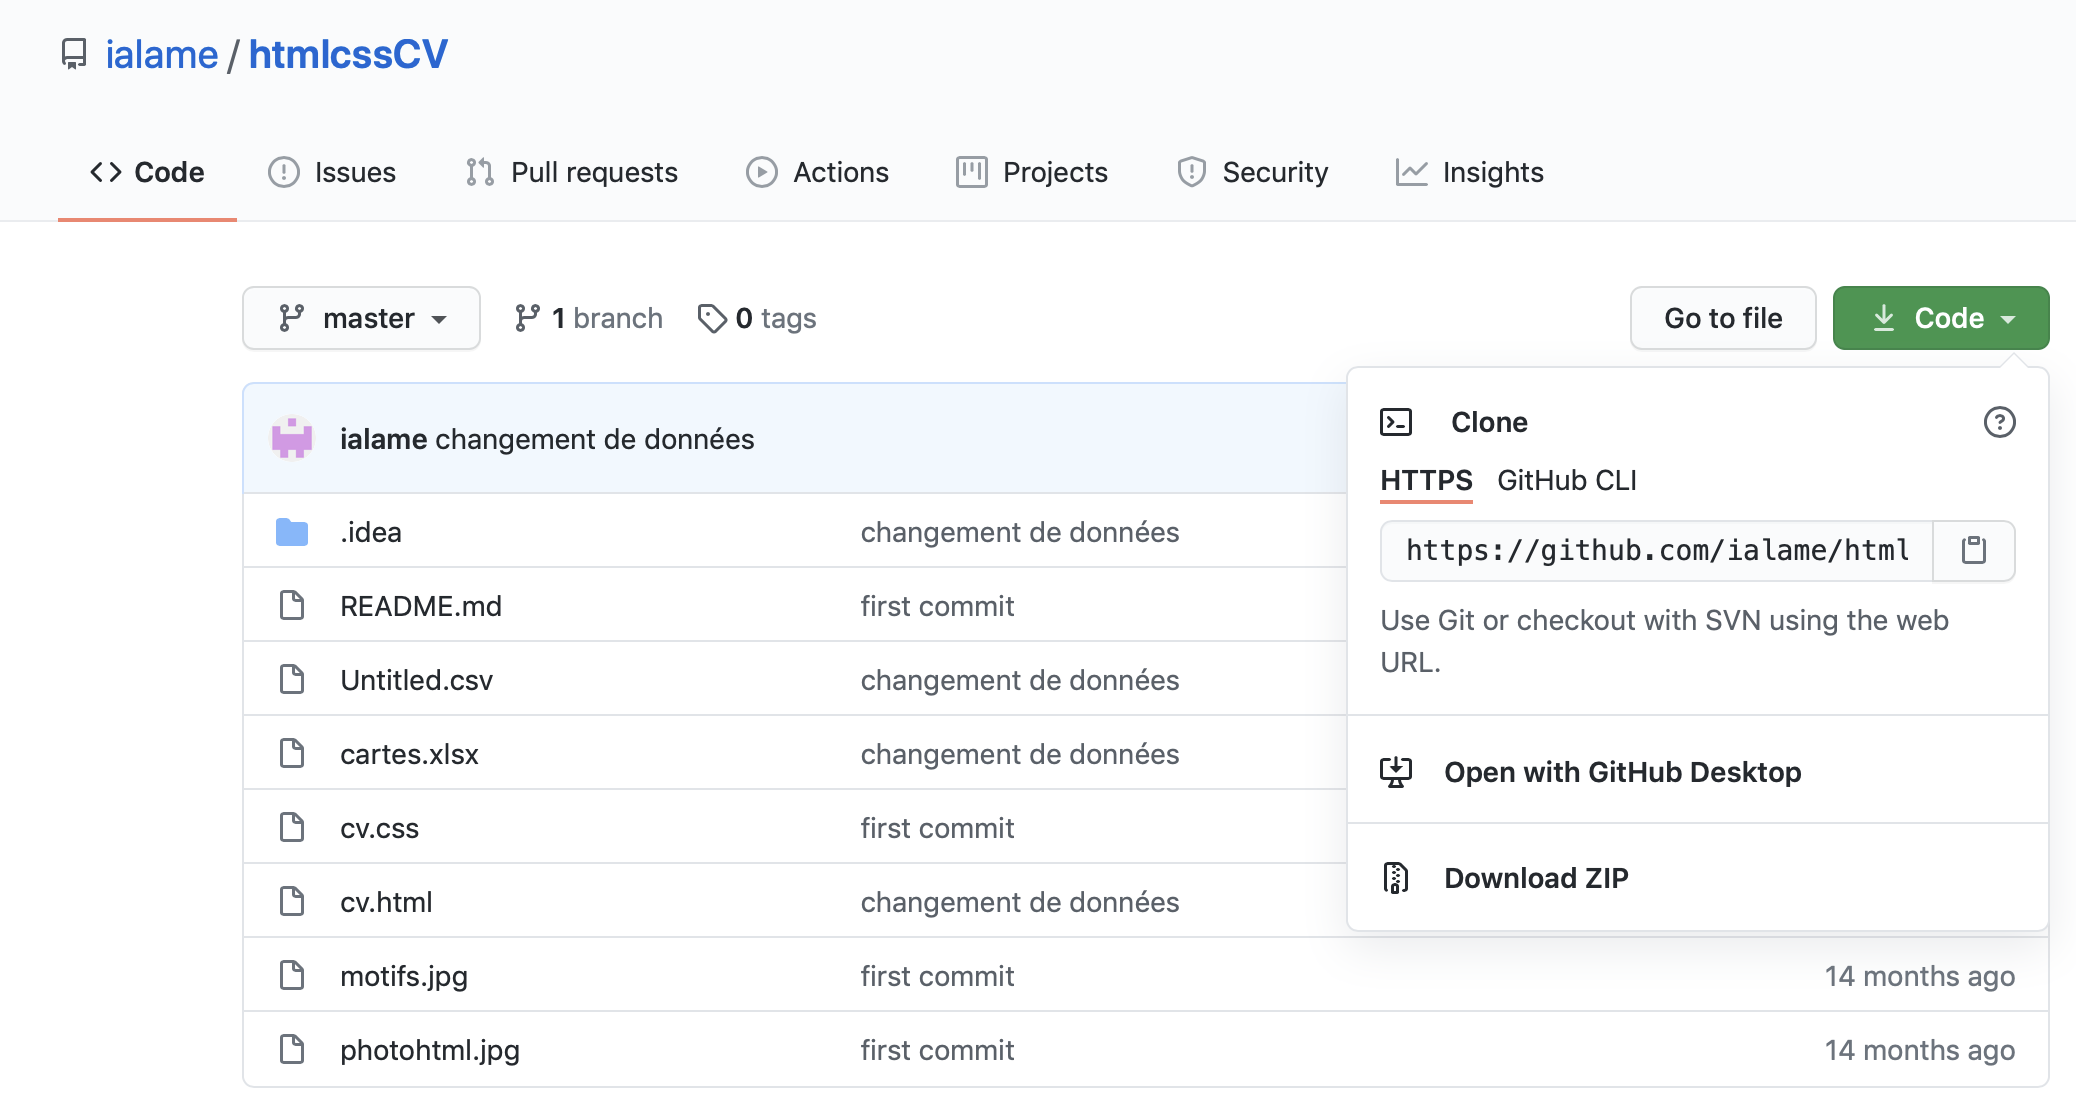
\includegraphics[scale=0.3]{git.png} 
\includegraphics[scale=0.14]{cv.png} 
\end{center}


\begin{enumerate}
\item Télécharger le dossier {\tt htmlcssCV} sous format zippé en cliquant sur {\tt code} puis {\tt Download ZIP}.
\item Modifier les données personnelles dans le fichier {\tt cv.html}  pour que cette page devient votre propre CV.
%\item Personnaliser l'apparence de votre CV en modifiant le fichier {\tt cv.css}.
\end{enumerate}

\section{Le parseur HTML : BeautifulSoup}
BeautifulSoup est une bibliothèque Python permettant de parser du HTML de manière très simple et de façon tolérante aux erreurs. 

Tester BeautifulSoup avec l'exemple suivant:
\\
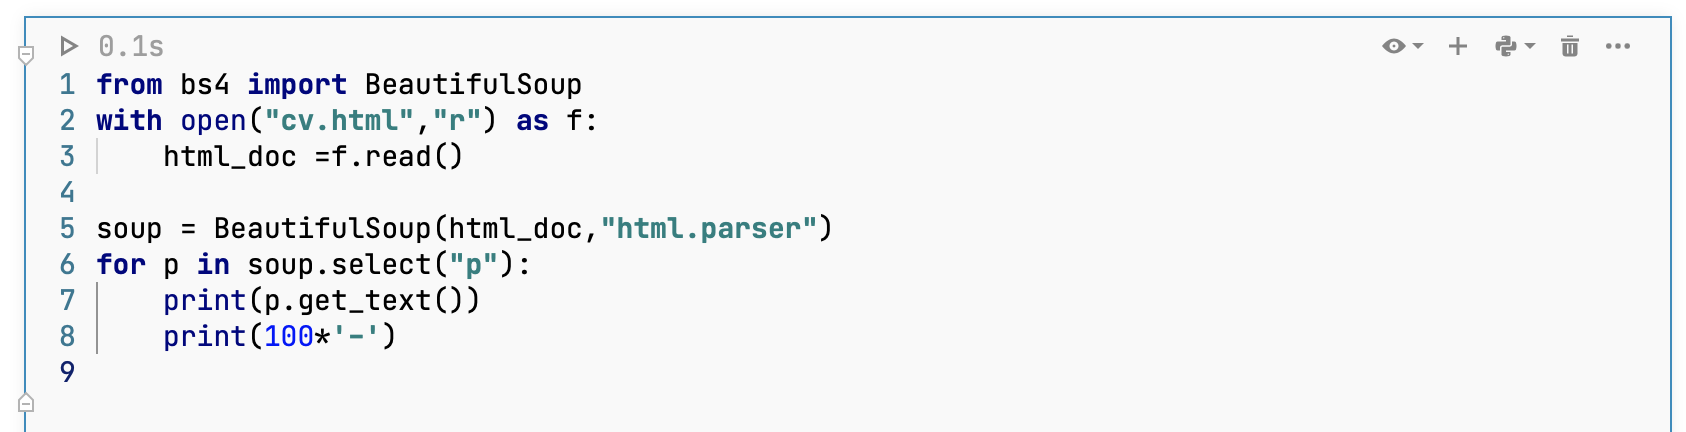
\includegraphics[scale=0.58]{pgm1.png} 
\\
On construit l'objet HTML parsé {\tt soup} à partir d'un filehandle  {\tt html\_doc} par l'instruction: 
\begin{verbatim}
   soup = BeautifulSoup(html_doc, "html.parser")
\end{verbatim}
où {\tt "html.parser"} est une option indiquant au constructeur {\tt BeautifulSoup} le format HTML et {\tt select("selecteur css")} est une méthode de la classe {\tt BeautifulSoup} qui retourne une liste d'objet balise correspondant au sélecteur css spécifié.  

Sur la page: {\tt https://www.crummy.com/software/BeautifulSoup/bs4/doc/} on trouve les méthodes de la classe BeautifulSoup les plus utiles.

A l'aide d'un programme python:
\begin{enumerate}
\item Lister les catégories du cv (les balises {\tt dt}).
\item Lister les sous titres H2 du cv.
\item Extraire du cv les activités de sa propriétaire à l'association "La Coco". 
\item Récupérer les coordonnées de Claire DELALUNE: Le nom, l'adresse, le téléphone, le mail et les langues vivantes.
\end{enumerate}
\section{Manipulation d'Excel en Python: openpyxl}
Installer, si nécessaire,  openpyxl avec les commandes suivantes:
\begin{center}
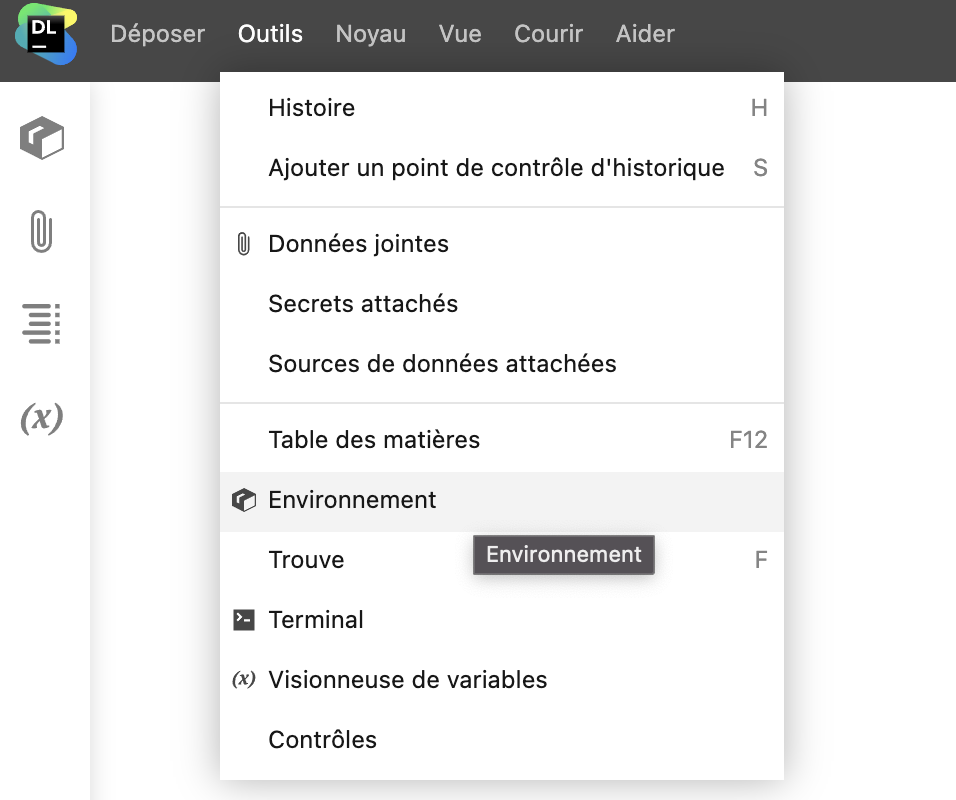
\includegraphics[scale=0.58]{environnement.png} 
\end{center}
\begin{center}
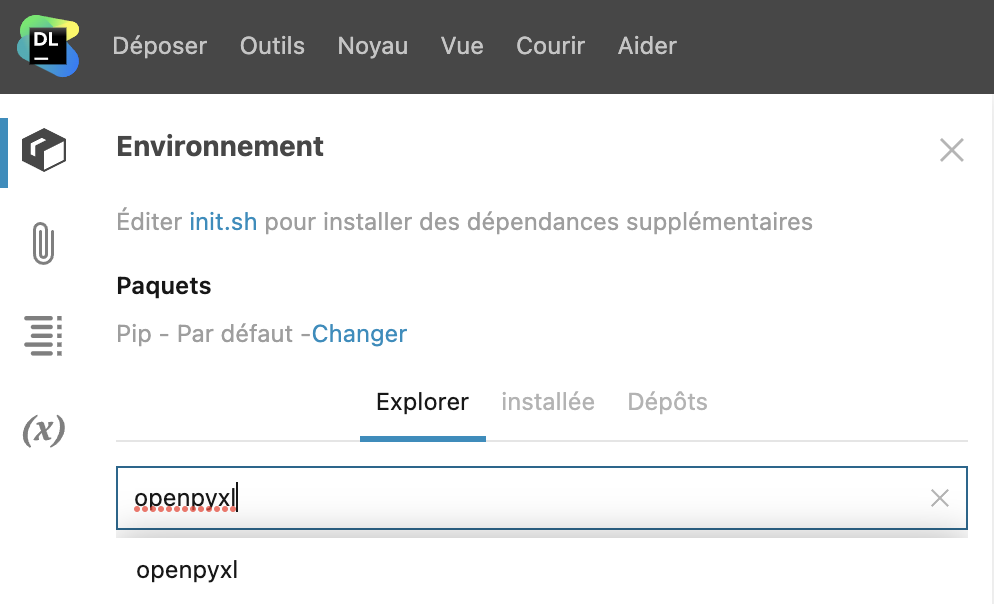
\includegraphics[scale=0.58]{openpyxl.png} 
\end{center}
\begin{center}
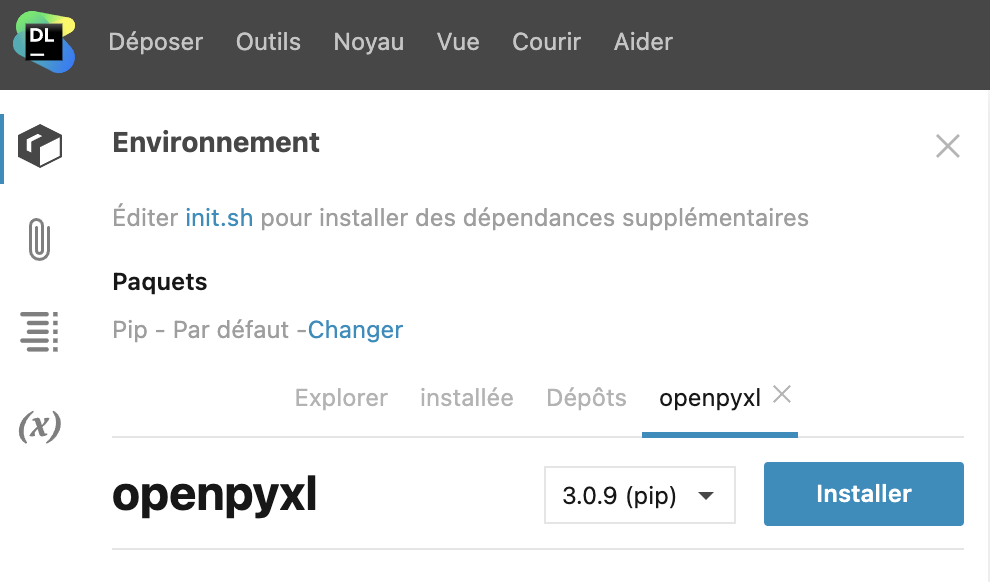
\includegraphics[scale=0.58]{openpyxl2.png} 
\end{center}

\begin{enumerate}
\item Ouvrir les fichier cartes.xlsx et afficher sur le console son contenu à l'aide du code suivant:

\begin{center}
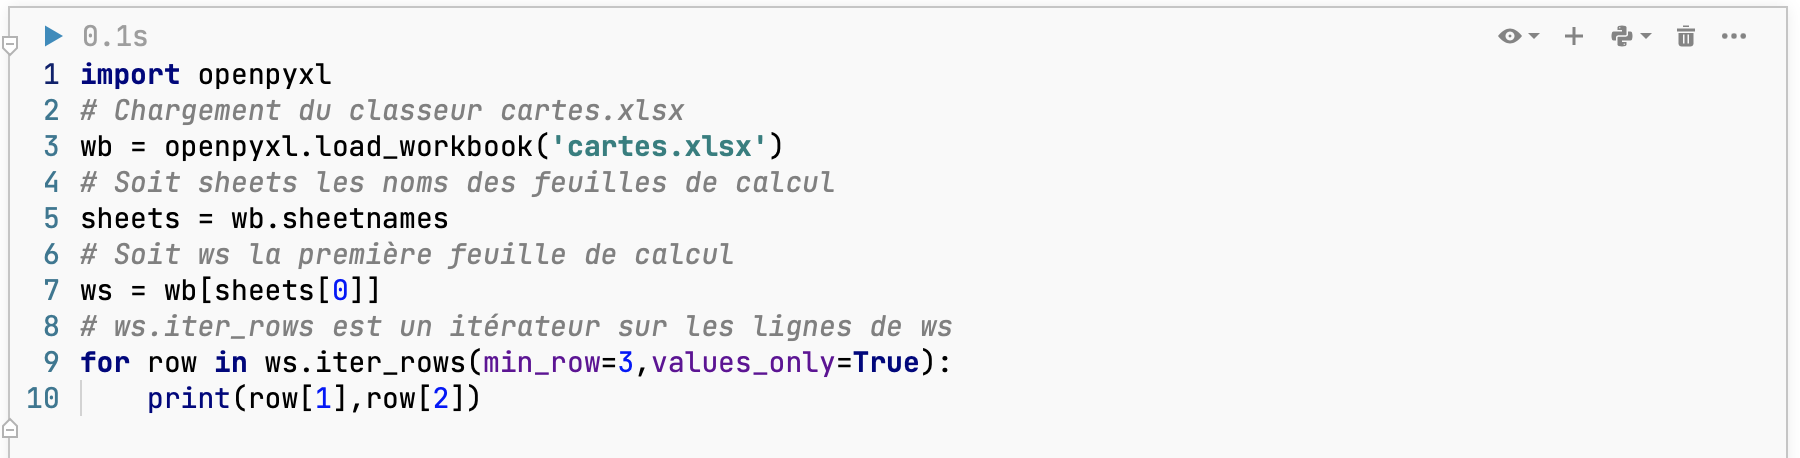
\includegraphics[scale=0.5]{pgm2.png} 
\end{center}


%\begin{verbatim}
%import openpyxl
%
%# Load in the workbook
%wb = openpyxl.load_workbook('cartes.xlsx')
%
%# Get sheet names
%sheets = wb.sheetnames
%ws = wb[sheets[0]]
%for row in ws.iter_rows(min_row=3,values_only=True):
%    print(row[1],row[2])
%\end{verbatim}

La méthode {\tt load\_workbook} de la classe {\tt openpyxl} permet d'ouvrir le fichier excel {\tt cartes.xlsx}. Le {\tt workbook} obtenu contient ses feuilles de calcul dans le tableau {\tt ws=wb.sheetnames}. On extrait la première feuille de calcul en faisant {\tt ws = wb[sheets[0]]}. La méthode {\tt iter\_rows} retourne un iterateur que l'on peut utiliser dans une boucle {\tt for} pour afficher les éléments d'une ligne courante.
\item Exécuter le programme suivant:
\begin{center}
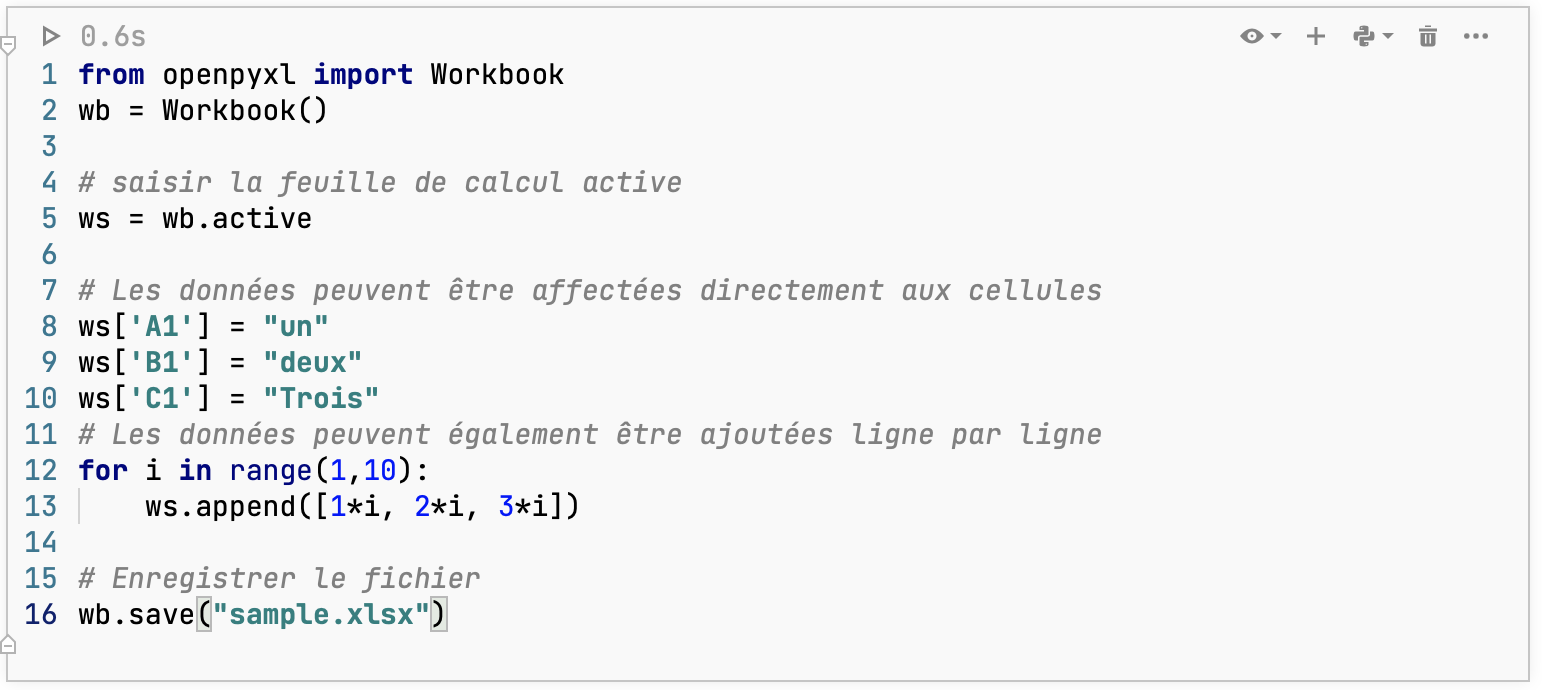
\includegraphics[scale=0.59]{pgm25.png} 
\end{center}


%\begin{verbatim}
%from openpyxl import Workbook
%wb = Workbook()
%
%# saisir la feuille de calcul active
%ws = wb.active
%
%# Les données peuvent être affectées directement aux cellules
%ws['A1'] = "un"
%ws['B1'] = "deux"
%ws['C1'] = "Trois"
%# Les données peuvent également être ajoutées ligne par ligne
%for i in range(1,10):
%    ws.append([1*i, 2*i, 3*i])
%
%# Enregistrer le fichier
%wb.save("sample.xlsx")
%\end{verbatim}

\end{enumerate}
\section{Importation des données à partir d'un site web}
On commence  par afficher le site web: {\tt https://www.ebay.fr}

chercher le produit {\tt Pikachu 58/102}

\begin{center}
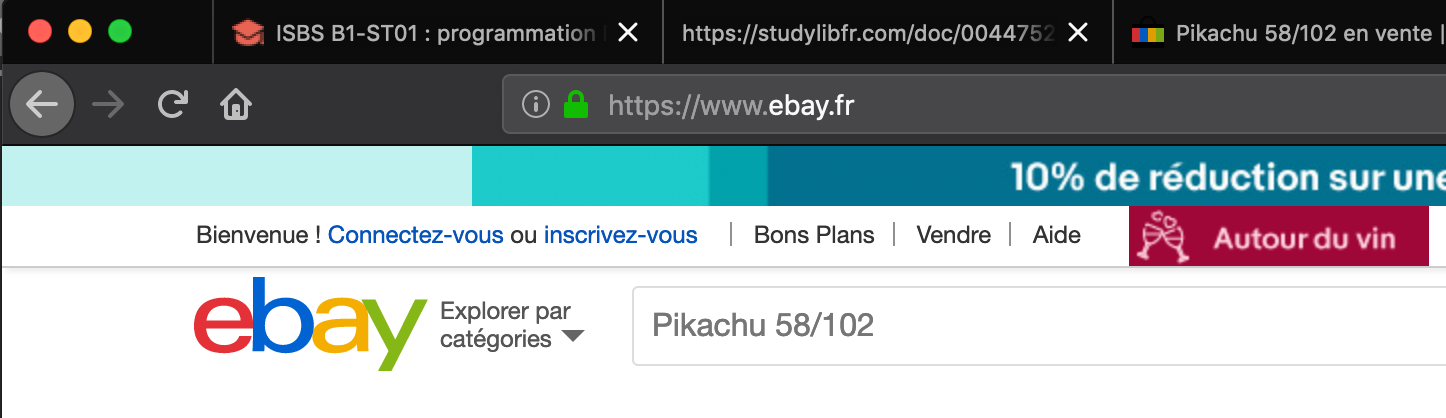
\includegraphics[scale=0.5]{ebay1.png} 
\end{center}
dans la colonne de gauche du site, filtrer la recherche en choisissant dans la rubrique {\tt Afficher uniquement} l'option {\tt Ventes réussies}
\begin{center}
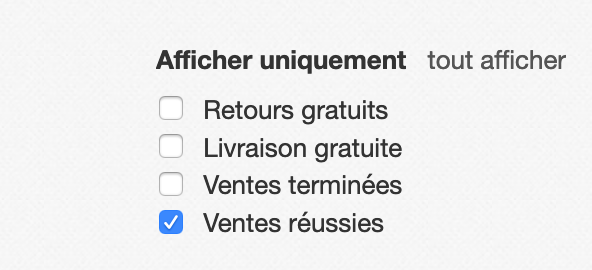
\includegraphics[scale=0.5]{ebay2.png} 
\end{center}
Vérifier bien que l'url de la page web courante du site ressemble à ceci:\\
{\tt https://www.ebay.fr/sch/i.html?\_from=R40\&\_sacat=0\&\_nkw=Pikachu\%2058/102\&LH\_Complete=1\&LH\_Sold=1\&rt=nc}

Remarquer que l'espace dans la chaîne de recherche {\tt Pikachu 58/102} a été remplacé par {\tt \%20}.

A présent, nous allons repérer le résultat de la recherche dans le fichier source HTML en cliquant sur le bouton droite de la souris et en choisissant Examiner l'élément dans le menu contextuelle.

\begin{center}
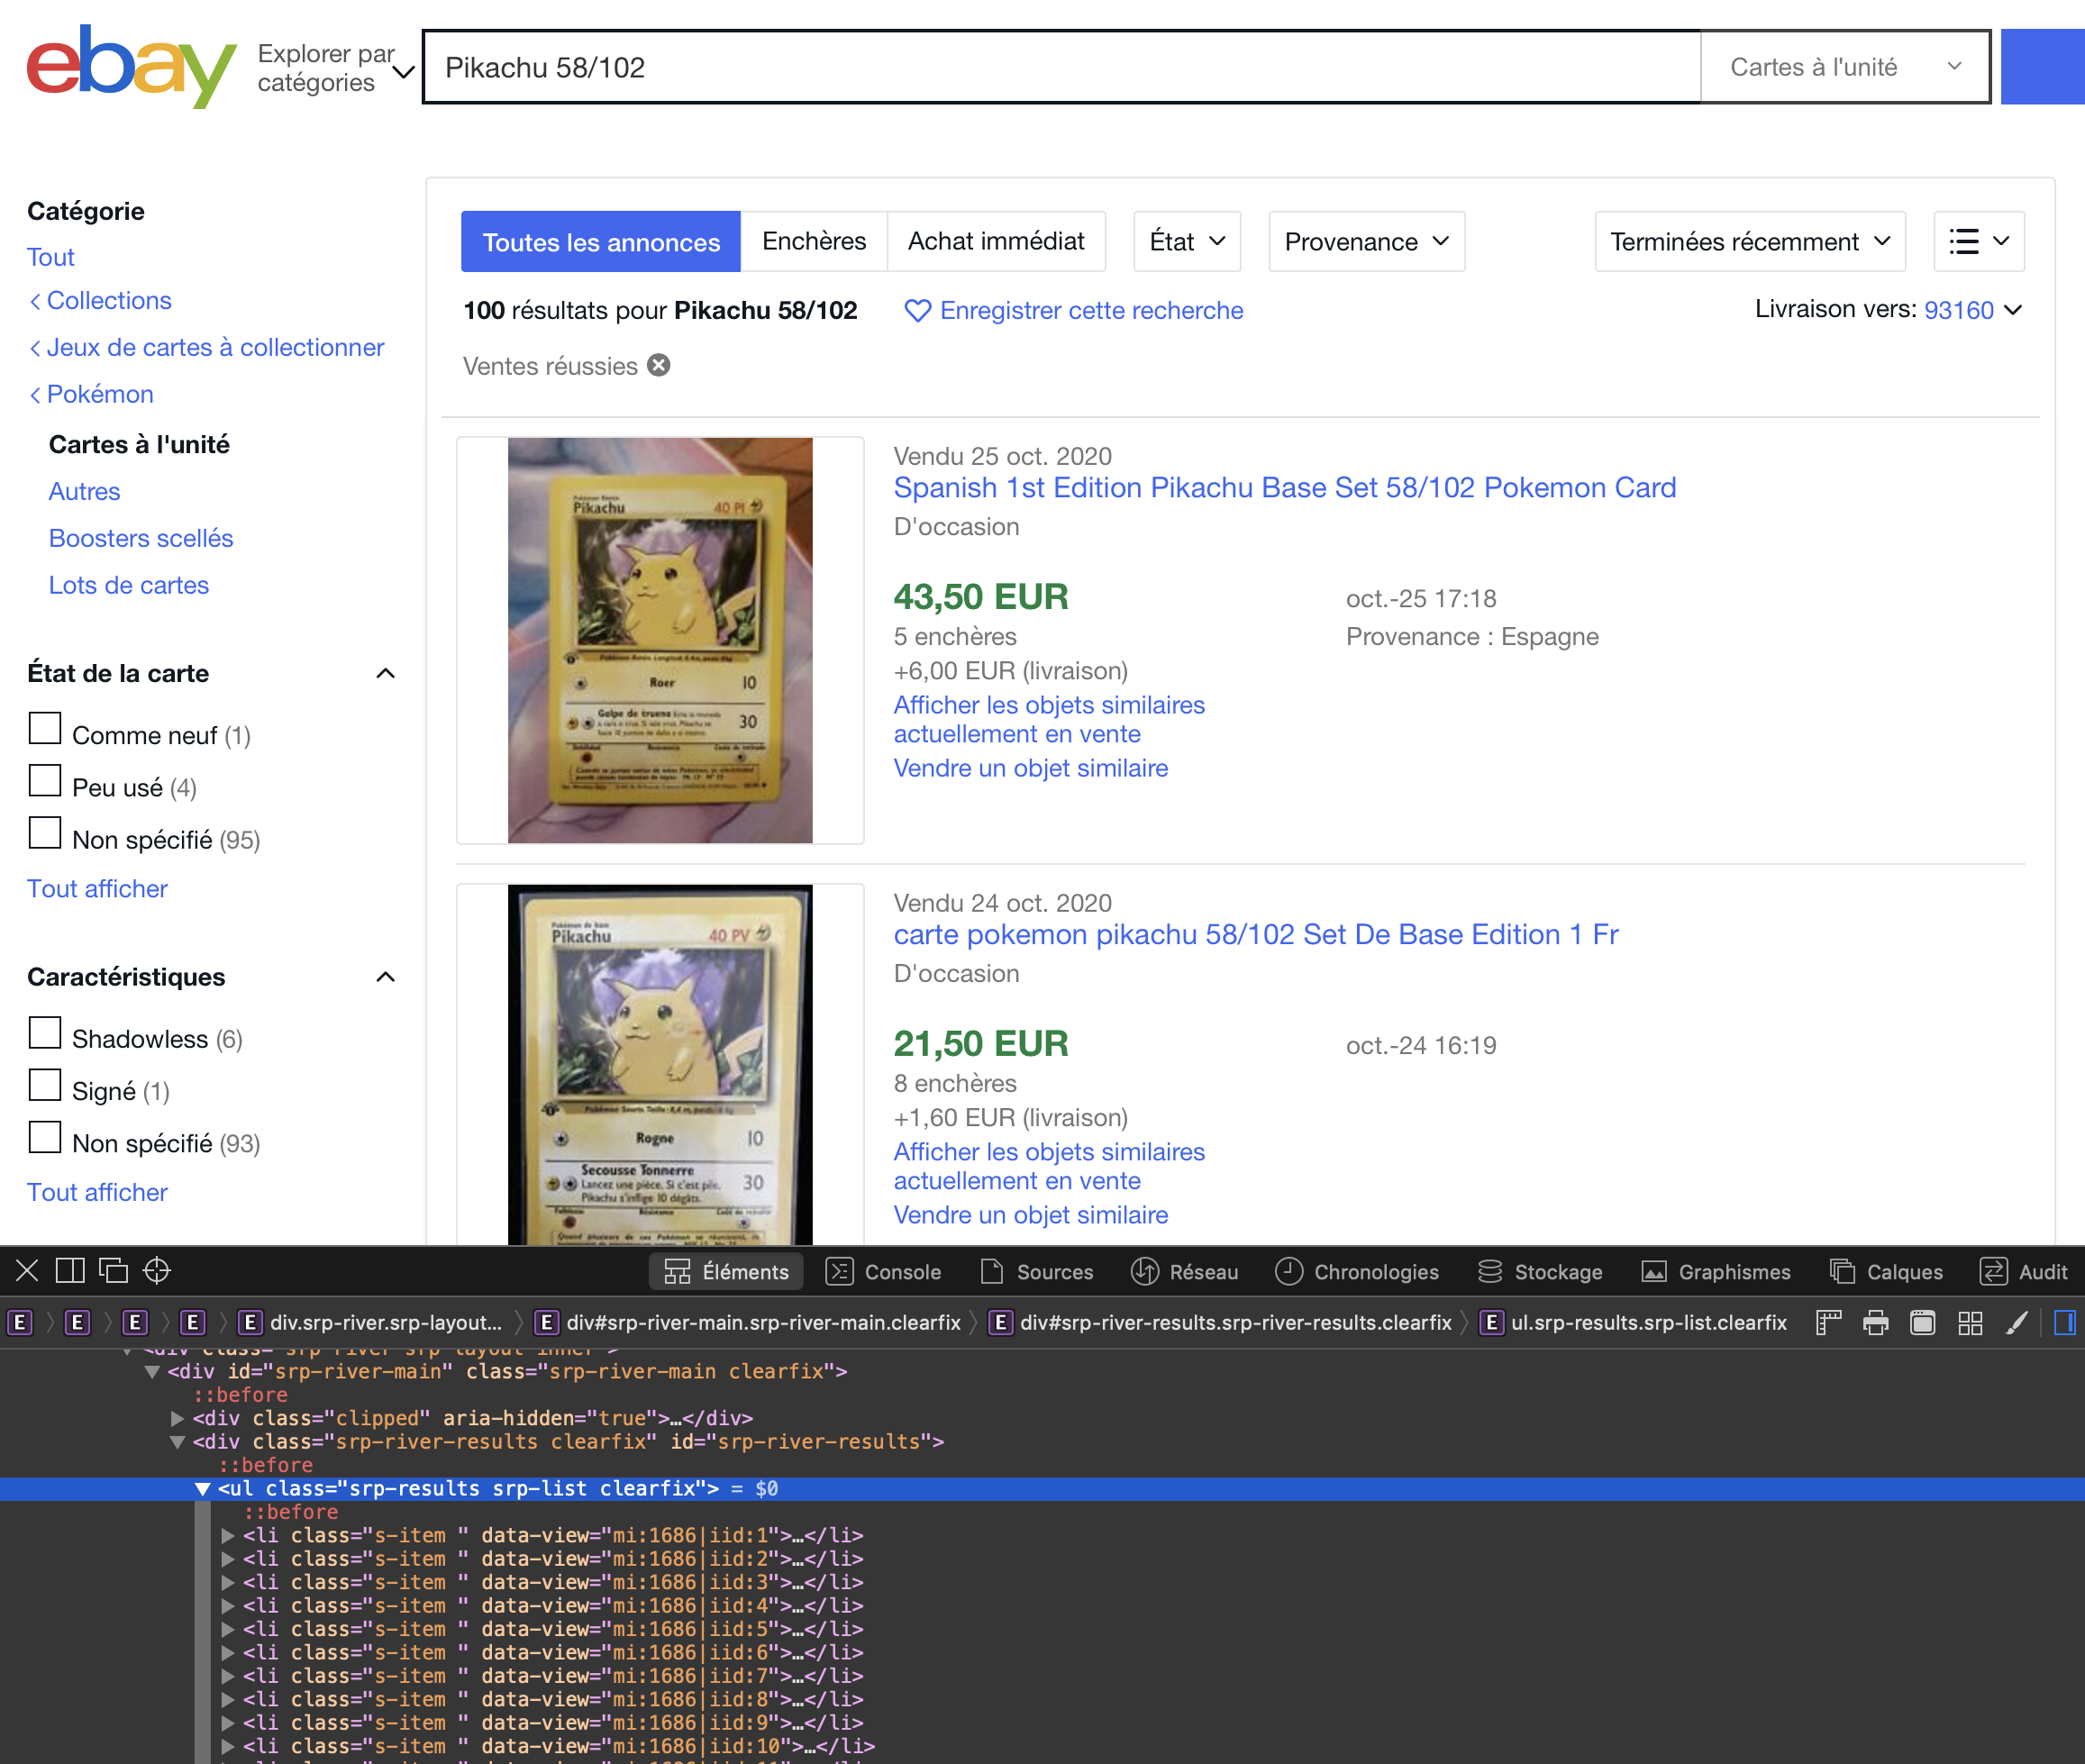
\includegraphics[scale=0.3]{ebay3.png} 
\end{center}

La liste des produits vendus {\tt <ul class="srp-results srp-list clearfix">}  est caractérisée par les trois classes {\tt srp-results, srp-list} et  {\tt clearfix}. Les éléments de cette liste {\tt <li>} sont caractérisés par la classe {\tt class="s-item"}. Donc, en python:
\begin{itemize}
\item On télécharge le document de la page web à l'aide de la méthode {\tt urllib.request.urlopen(url)}
\item A l'aide de la classe {\tt BeautifulSoup} on parse le document HTML: {\tt soup = BeautifulSoup(html\_doc, "html.parser")}
\item On cherche dans le document parsé l'ensemble de produits vendus par {\tt soup.select("li.s-item")[1:])} puis on affiche la liste avec une simple boucle {\tt for}.

\end{itemize}

 D'où le code python suivant:

\begin{center}
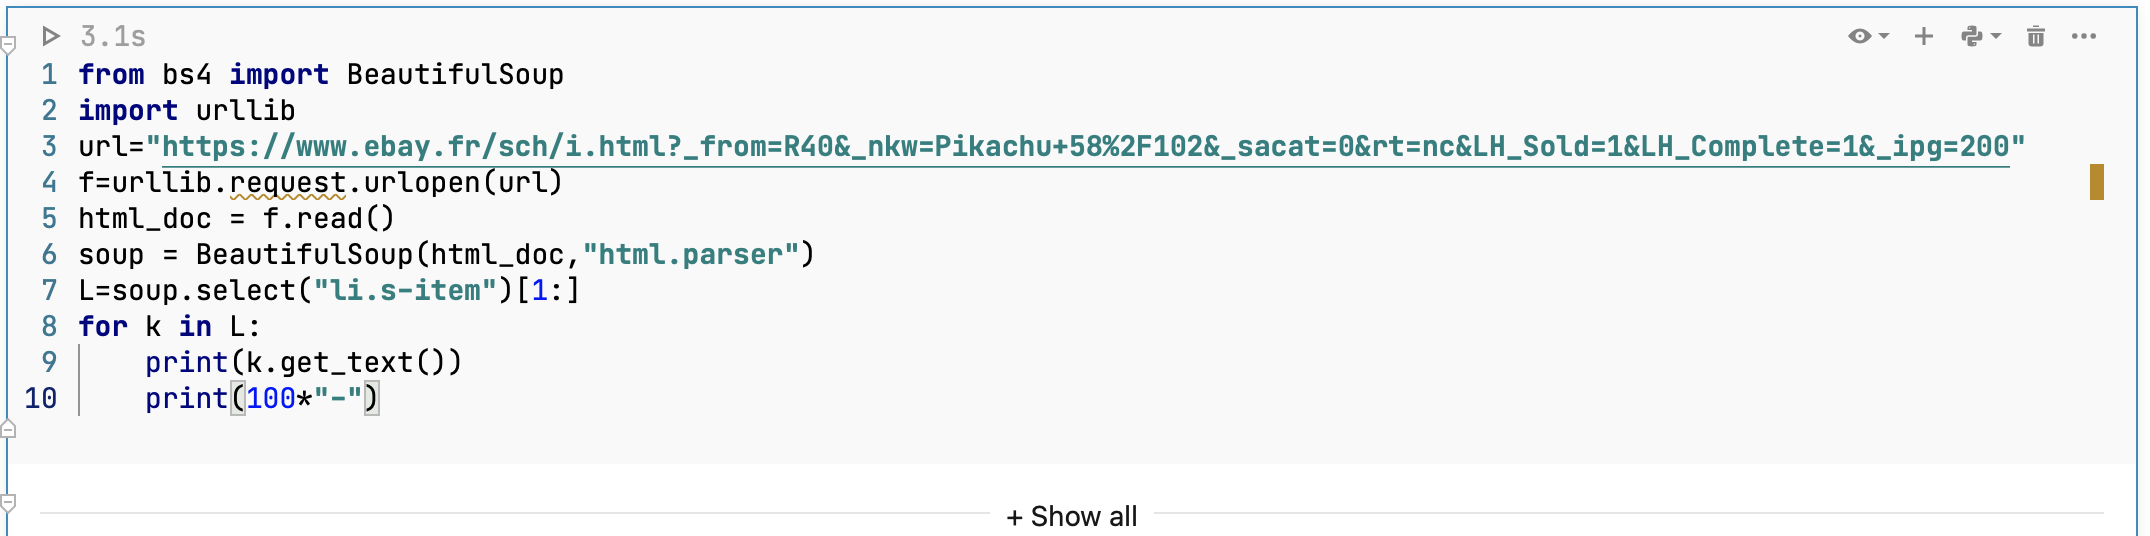
\includegraphics[scale=0.45]{pgm3.png} 
\end{center}

On cherche à extraire pour chaque produit vendu: 
\begin{center}
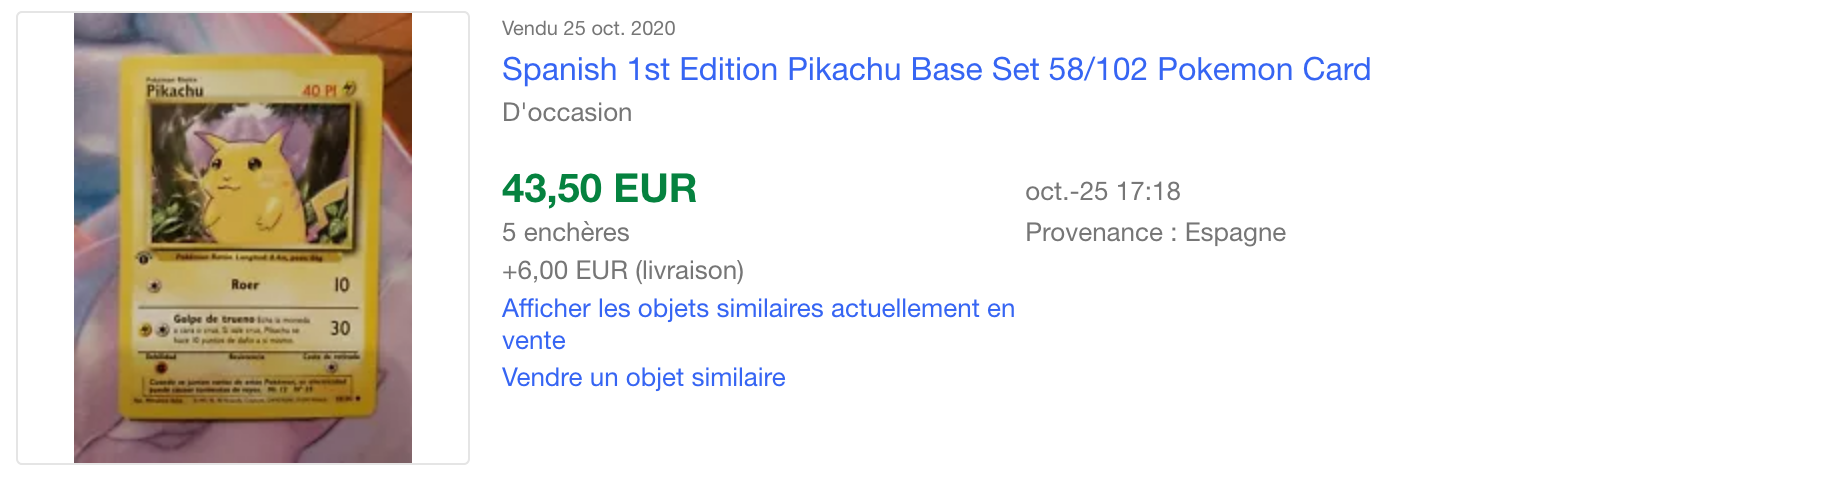
\includegraphics[scale=0.5]{ebay4.png} 
\end{center}

\begin{itemize}
\item Le titre, exemple: {\tt Spanish 1st Edition Pikachu Base Set 58\/102 Pokemon Card},
\item Le prix, exemple {\tt 43,50 EUR},
\item La date, exemple {\tt oct.-25 17:18}
\item La Provenance, exemple {\tt  Espagne}
\end{itemize}

Il suffit pour cela de repérer la donnée dans le fichier source HTML et d'appliquer une méthode de sélection convenable:
\begin{center}
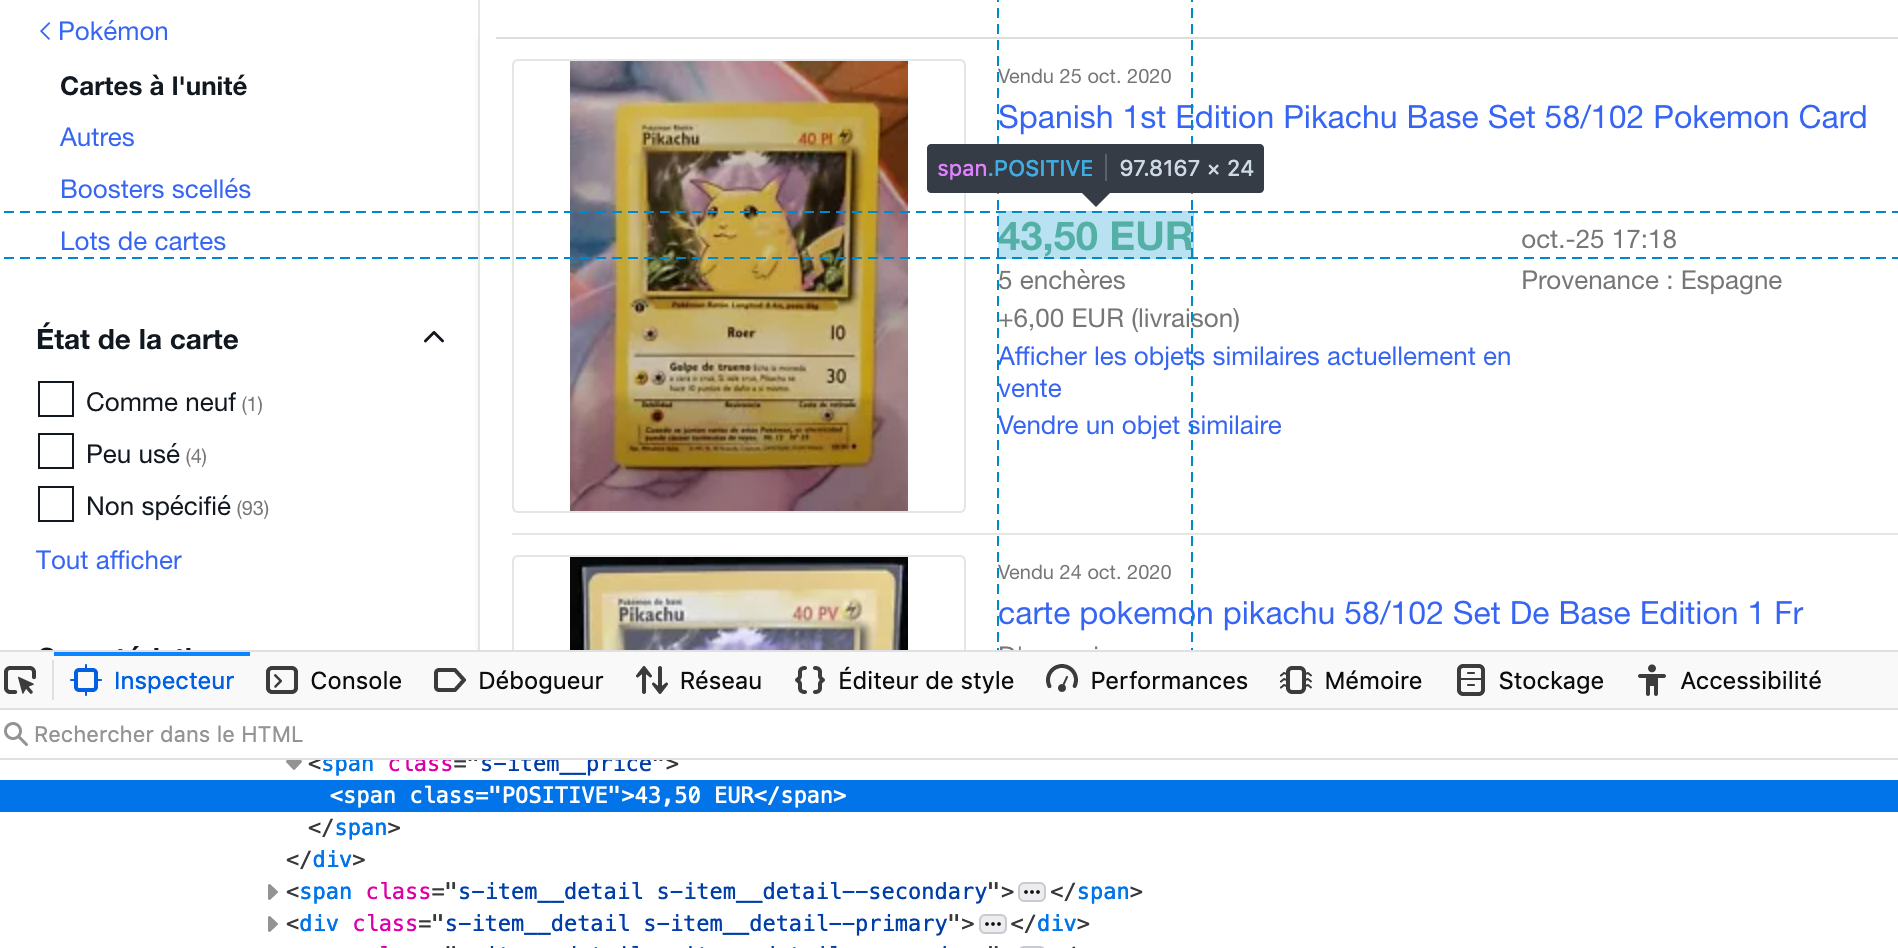
\includegraphics[scale=0.5]{ebay5.png} 
\end{center}
Par exemple le prix est un {\tt <span>} de classe {\tt POSITIVE} dans un {\tt <span>} de classe {\tt s-item\_\_price} . d'où l'instruction python:

\begin{verbatim}
prix=k.select(".s-item__price.POSITIVE")
prix=prix[0].text
\end{verbatim}
il en est de même pour les autres données:
\begin{center}
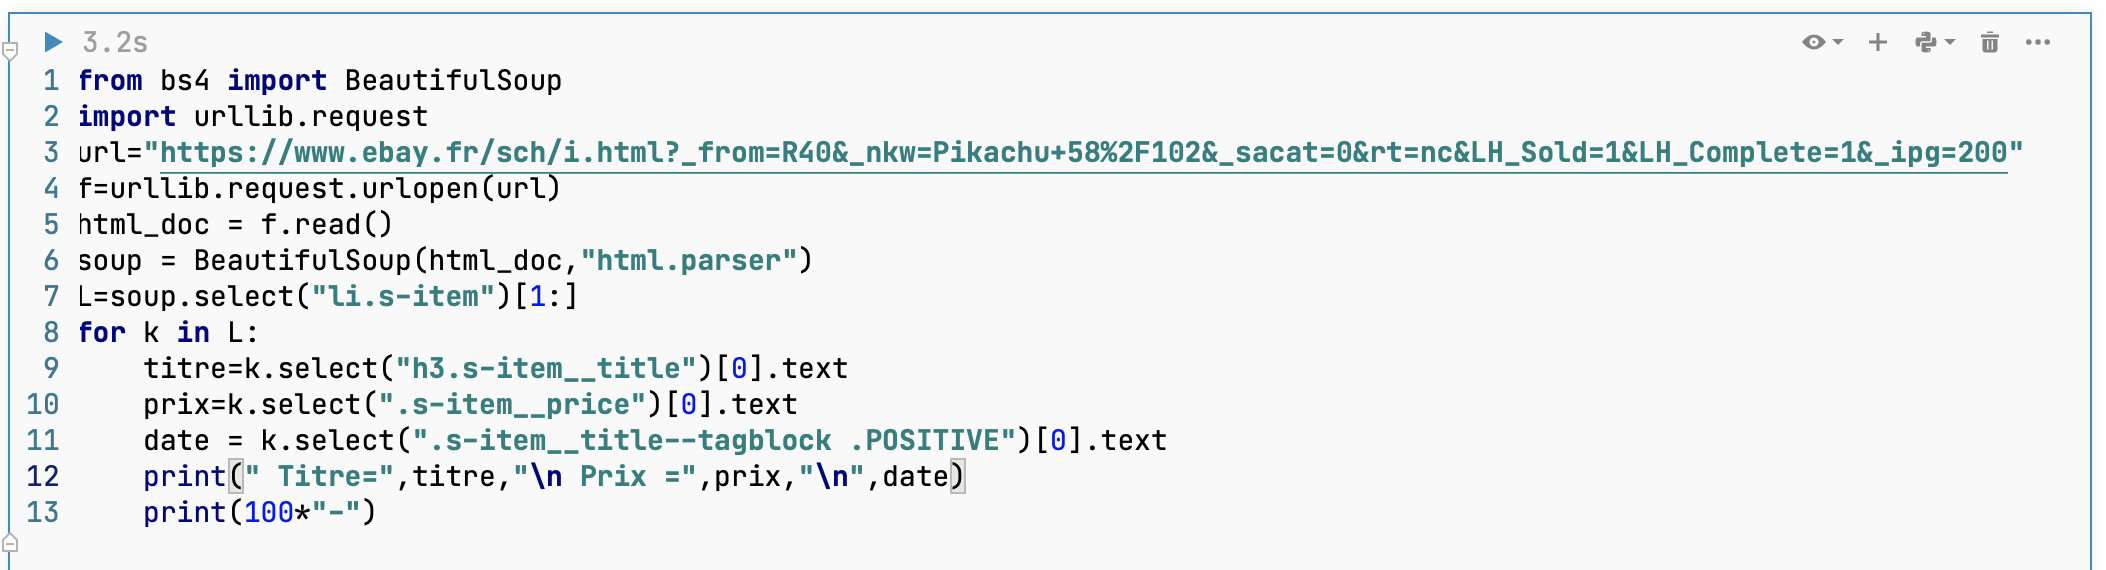
\includegraphics[scale=0.47]{pgm5.png} 
\end{center}
Attention: à rectifier dans ce code: {\tt div} à la place de  {\tt h3} à la ligne 9.
\begin{enumerate}
\item Ce programme récupère les données de la page web concernant les ventes de l'article {\tt Pikachu 58/102}. Compléter le code pour  sauvegarder le résultat dans un fichier excel {\tt ventes1.xlsx}.
\item Écrire une fonction {\tt parseDate} permettant de transformer une chaine de caractères de type: "Vendu  25 sept. 2021" en une date de type {\tt datetime64}.
\begin{center}
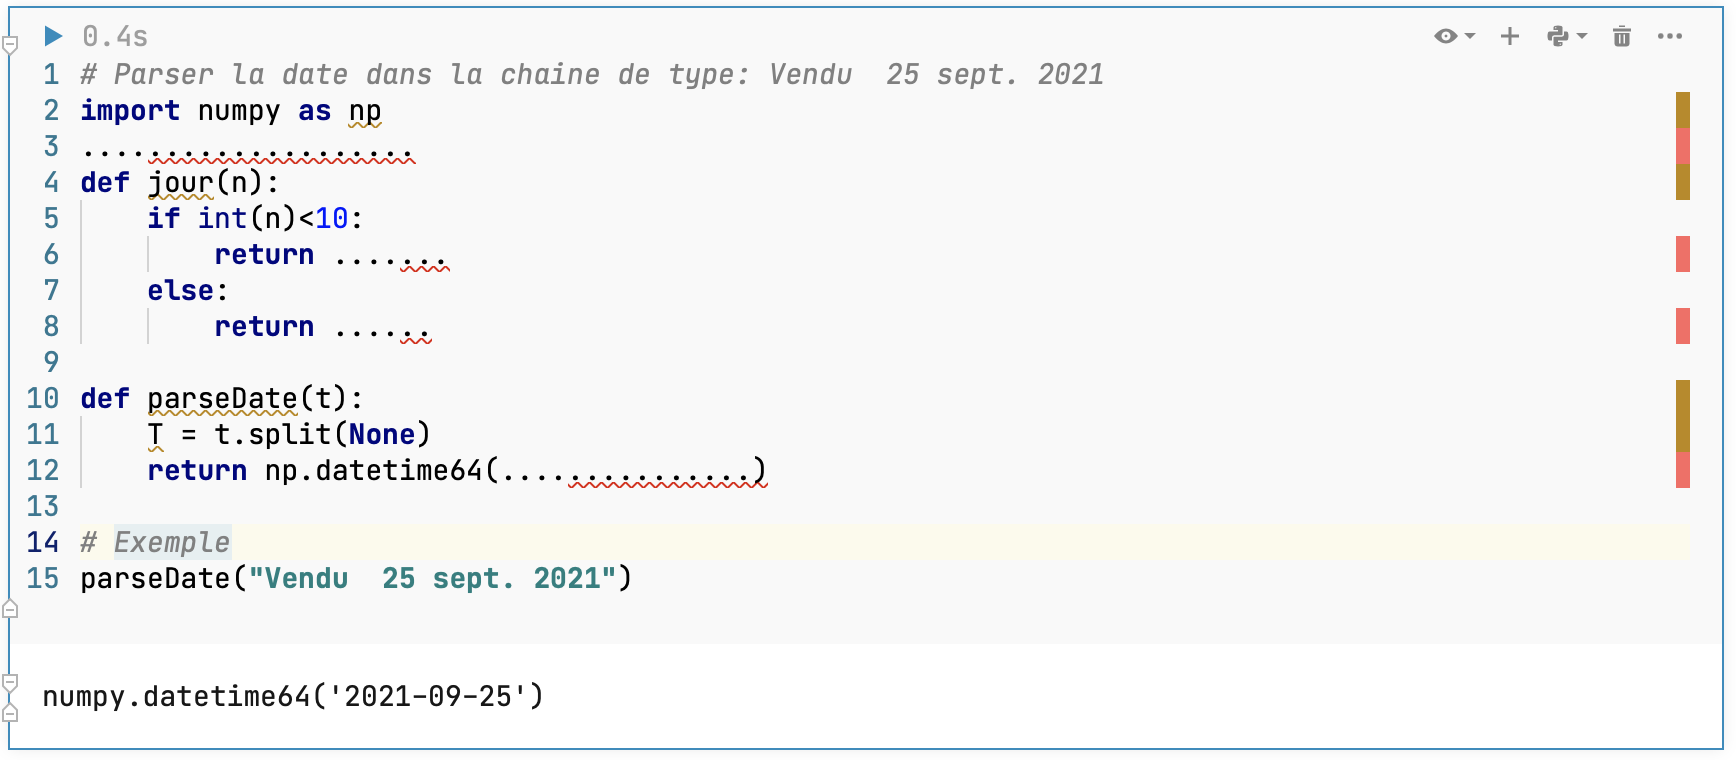
\includegraphics[scale=0.53]{pgm6.png} 
\end{center}
\item Écrire une fonction {\tt getPrix} permettant de transformer une chaine de caractères de type "41,82 EUR" en un nombre réel 41.82
\item Construire une série temporelle de type {\tt pandas.Series} indexant par date le prix de vente des cartes Pikachu 58/102:
\begin{center}
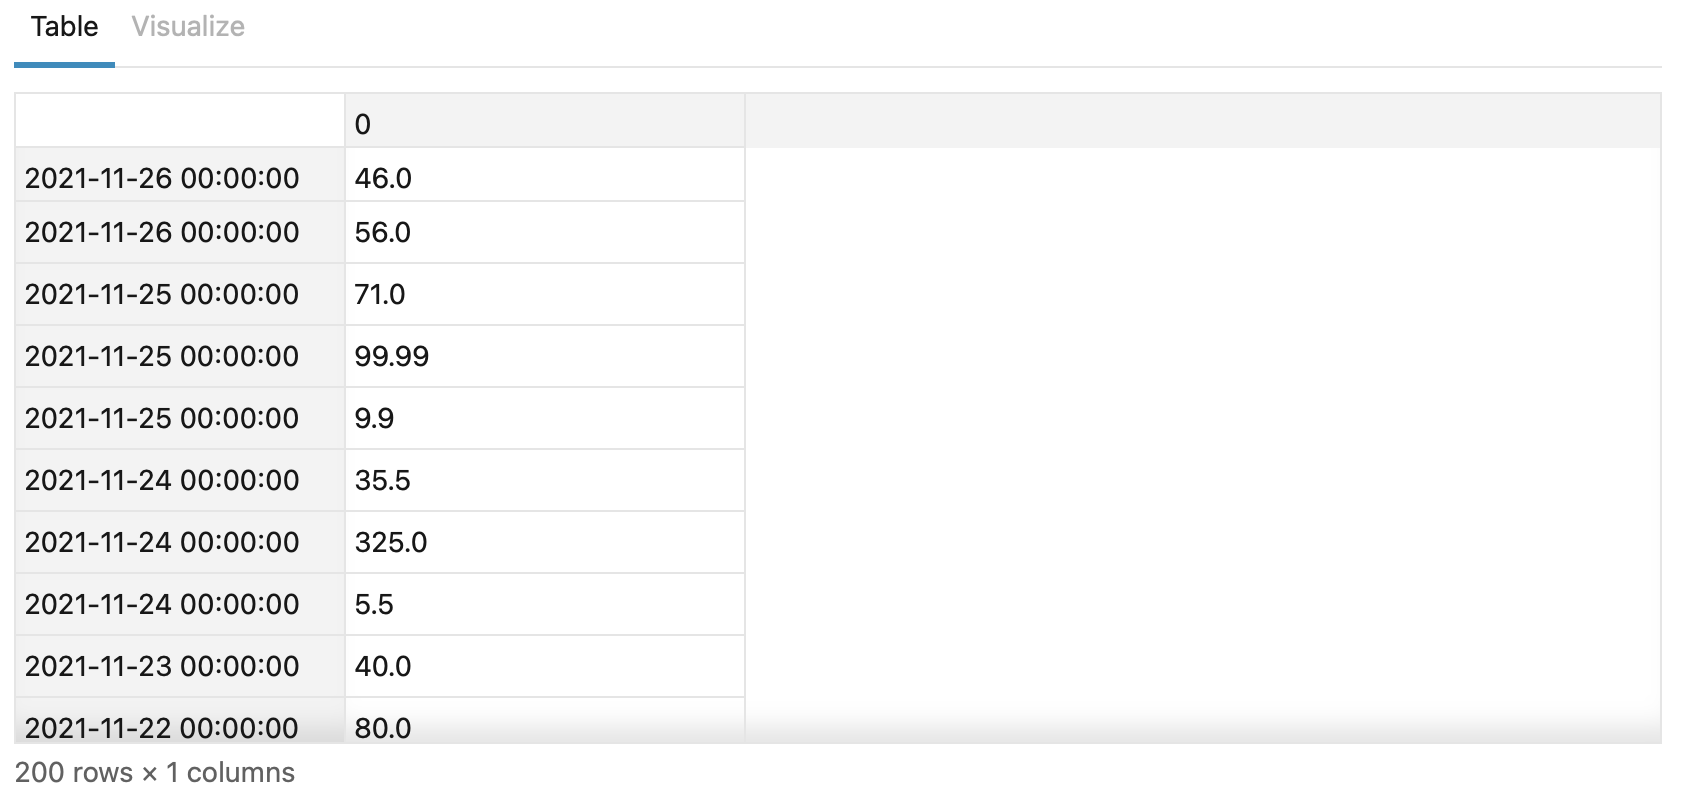
\includegraphics[scale=0.53]{serieTemporelleS.png} 
\end{center}
\item  Afficher les caractéristiques statistiques des ventes à l'aide la méthode {\tt describe()} puis représenter graphiquement l'évolution du prix en fonction du temps.
\end{enumerate}
\end{document}